\section{Разделение ip-адресов на подсети}

\begin{table}[H]
    \centering
    \caption{Разделение на подсети}
    \label{tab:networks}
    \begin{tabular}{|p{0.8cm}|p{1cm}|p{3cm}|p{3cm}|p{3cm}|p{3.2cm}|}
        \hline
        Но-мер под-се-ти & Ко-ли-чест-во хос-тов & ip подсети & Диапазон адресов & Широкове-щательный адрес & Маска под-сети \\
        \hline
        1 & 30 & 192.168.19.0 & 192.168.19.1-192.168.19.30 & 192.168.19.31 & 255.255.255.224 (/27) \\
        \hline
        2 & 6 & 192.168.19.64 & 192.168.19.65-192.168.19.70 & 192.168.19.71 & 255.255.255.248 (/29) \\
        \hline
        3 & 2 & 192.168.19.80 & 192.168.19.81-192.168.19.82 & 192.168.19.83 & 255.255.255.252 (/30) \\
        \hline
        4 & 6 & 192.168.19.72 & 192.168.19.73-192.168.19.78 & 192.168.19.79 & 255.255.255.248 (/29) \\
        \hline
        5 & 30 & 192.168.19.32 & 192.168.19.33-192.168.19.62 & 192.168.19.63 & 255.255.255.224 (/27) \\
        \hline
    \end{tabular}
\end{table}

\section{Работающая схема}

\begin{figure}[H]
    \centering
    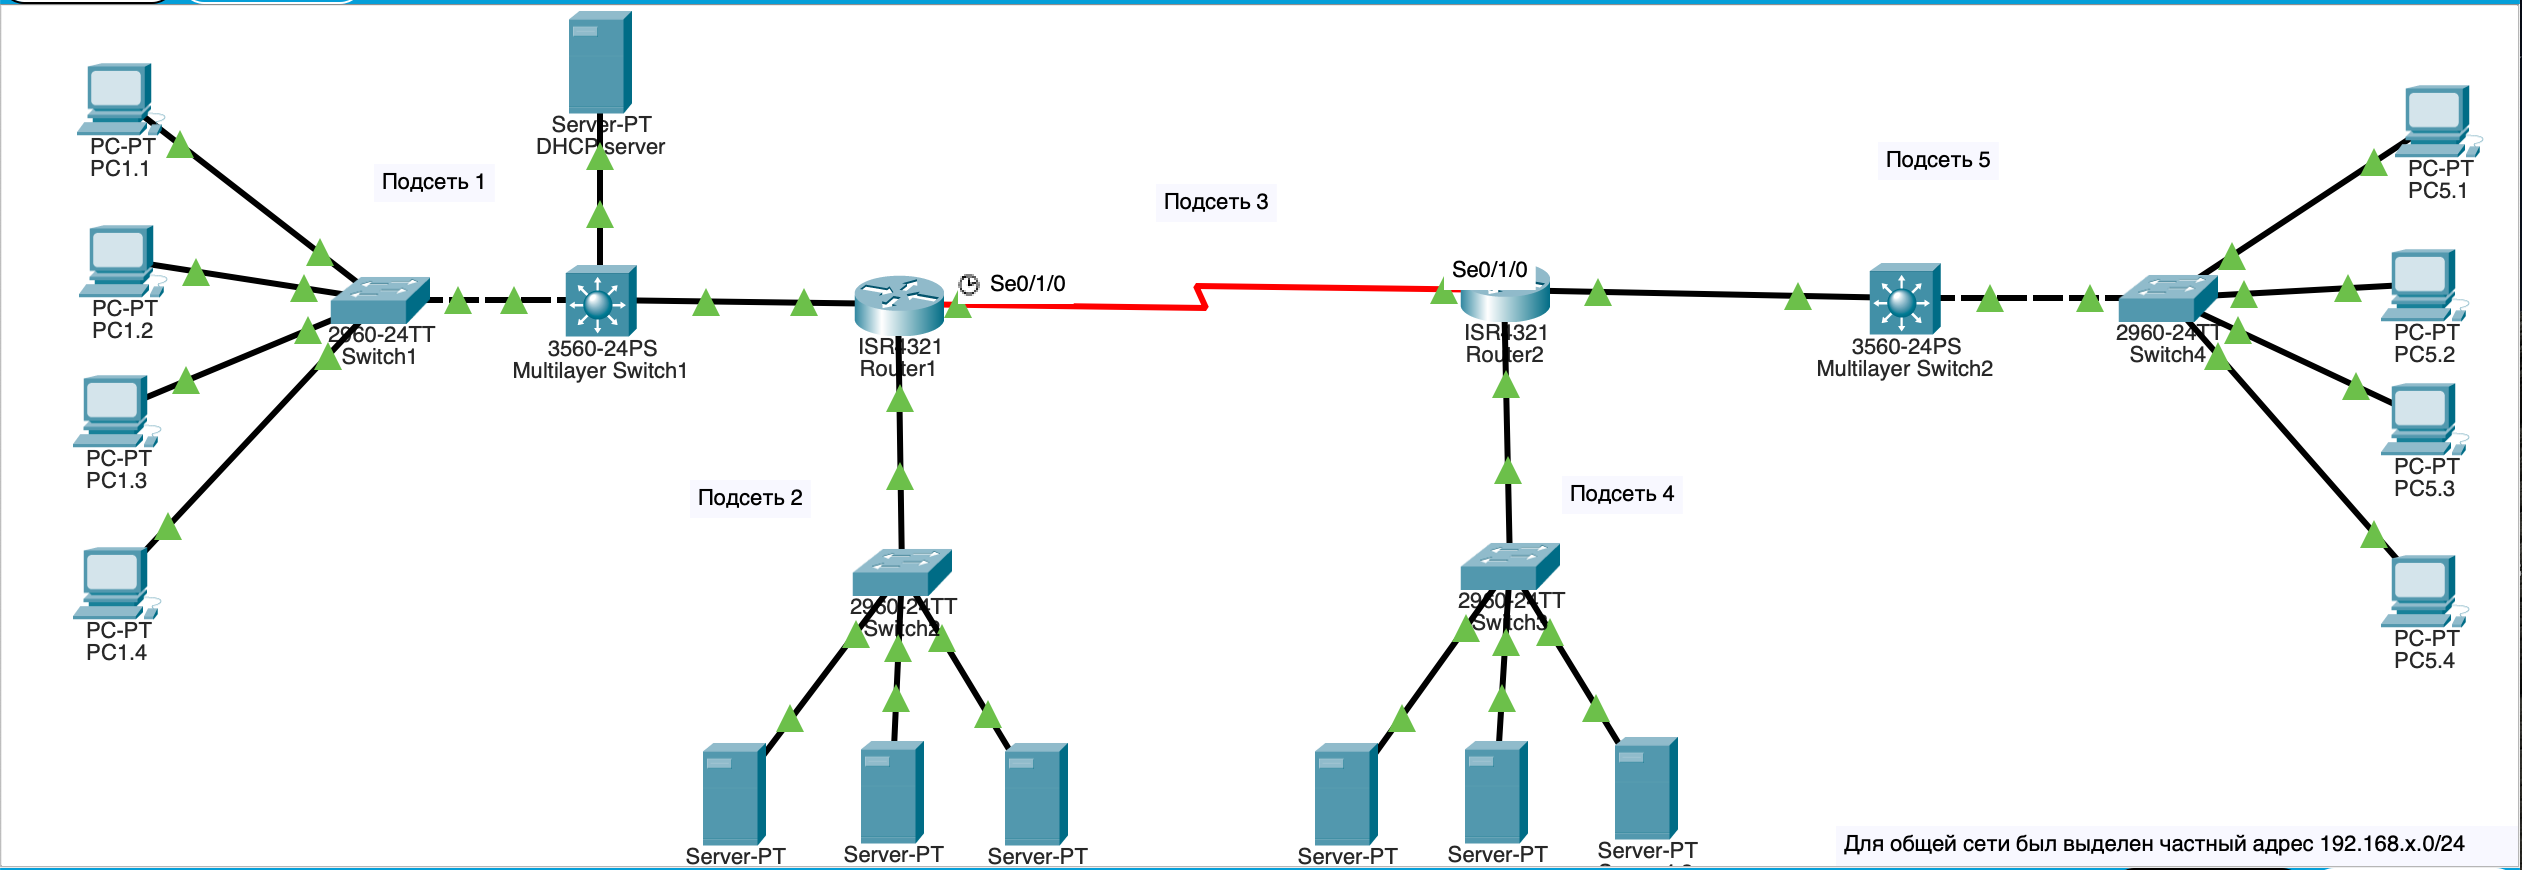
\includegraphics[width=0.8\textwidth]{img/content/schema.png}
    \caption{Схема с настроенными подсетями}
\end{figure}

\section{Настройка DHCP серверов}

\begin{figure}[H]
    \centering
    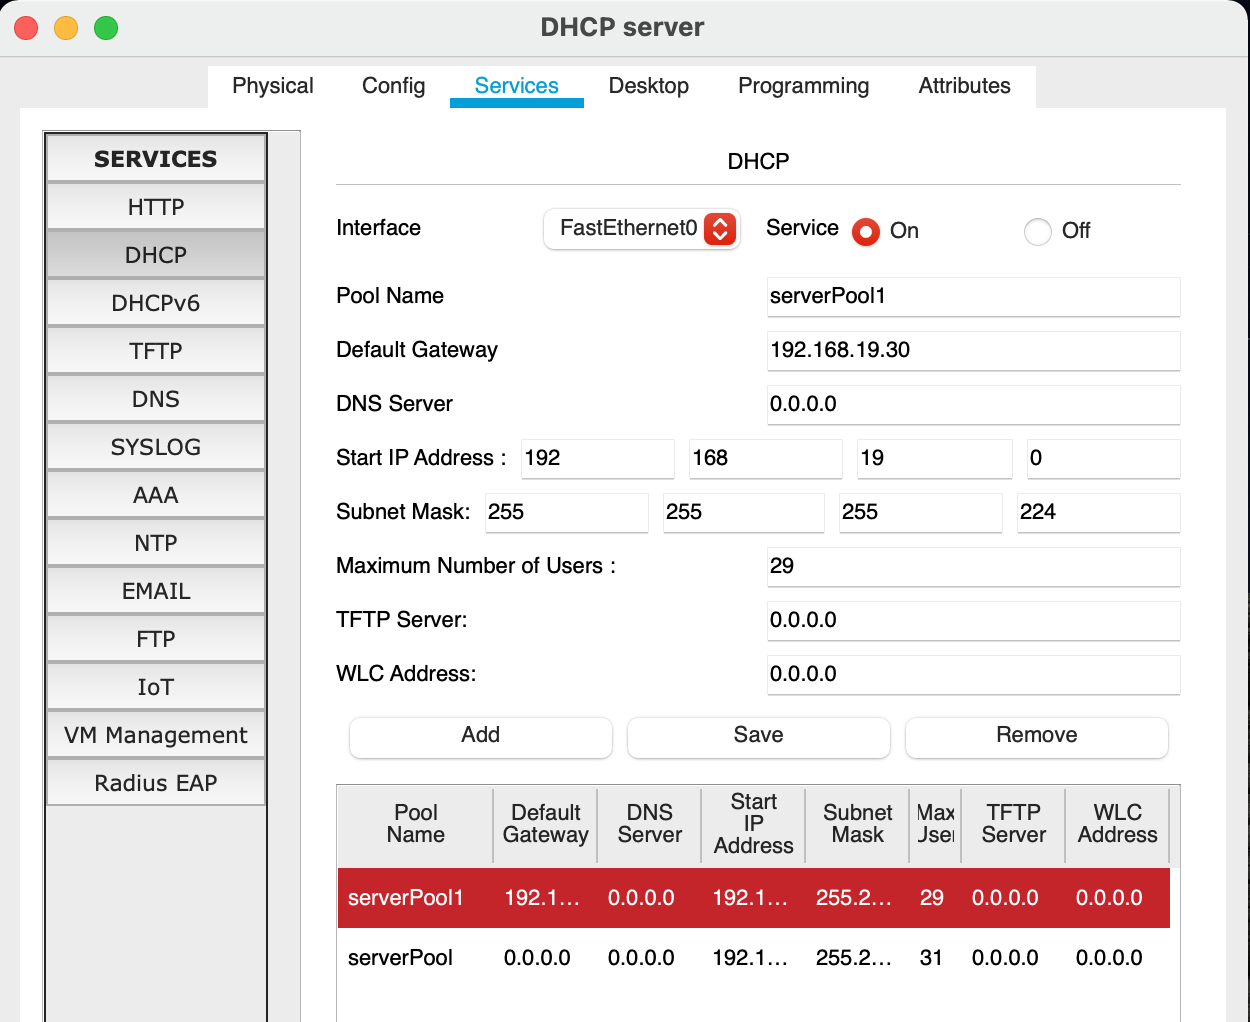
\includegraphics[width=0.5\textwidth]{img/content/DHCP_1.png}
    \caption{Настройка DHCP-сервера для первой подсети}
\end{figure}

\begin{figure}[H]
    \centering
    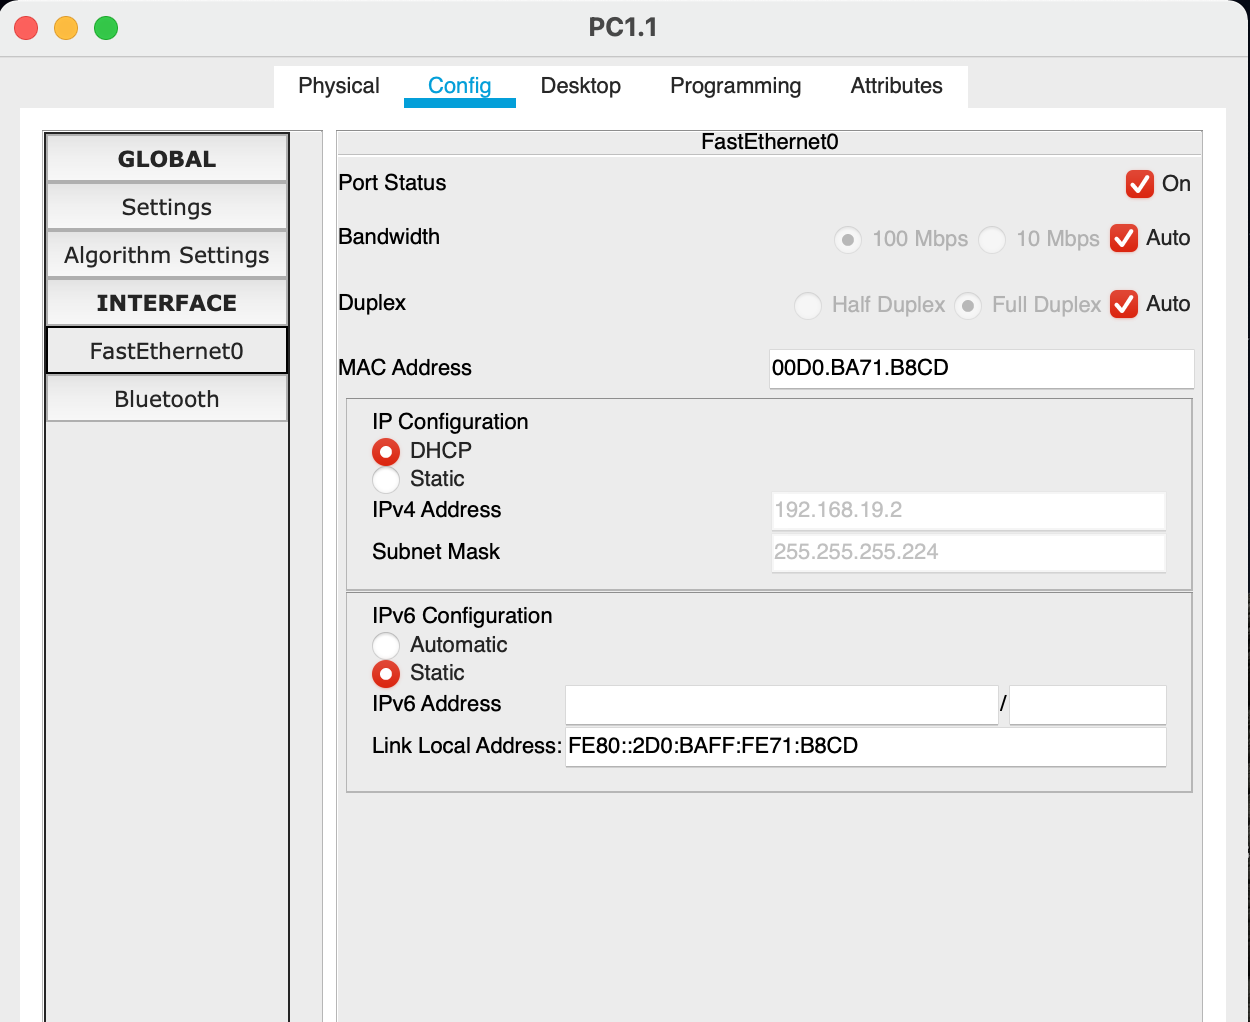
\includegraphics[width=0.5\textwidth]{img/content/PC_1.png}
    \caption{Автоматически выданный ip-адрес компьютера в первой подсети}
\end{figure}

\begin{figure}[H]
    \centering
    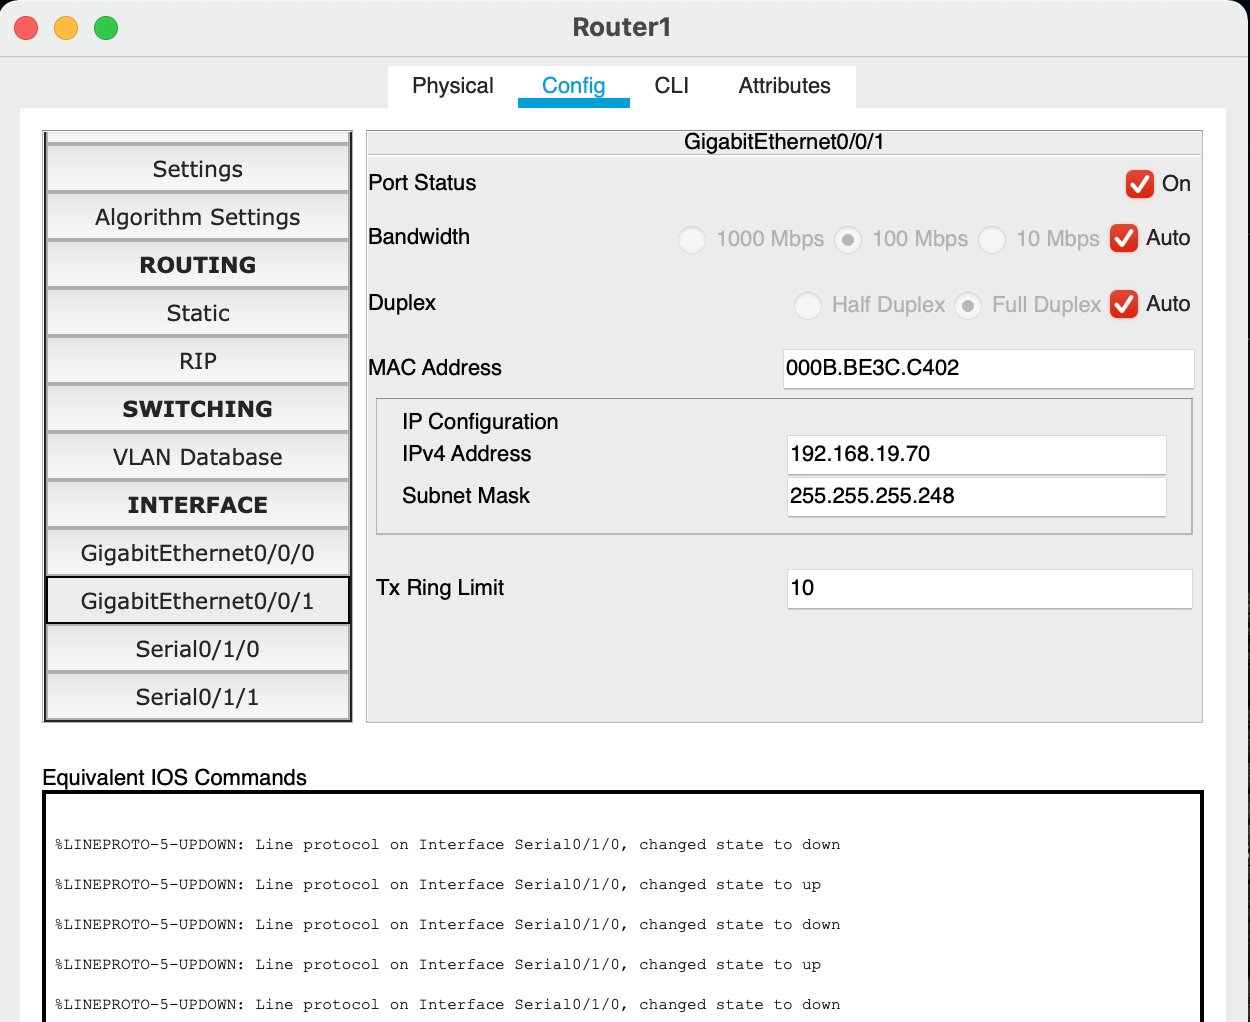
\includegraphics[width=0.5\textwidth]{img/content/DHCP_2.png}
    \caption{Настройка маршрутизатора в качестве DHCP-сервера для второй подсети}
\end{figure}

\begin{figure}[H]
    \centering
    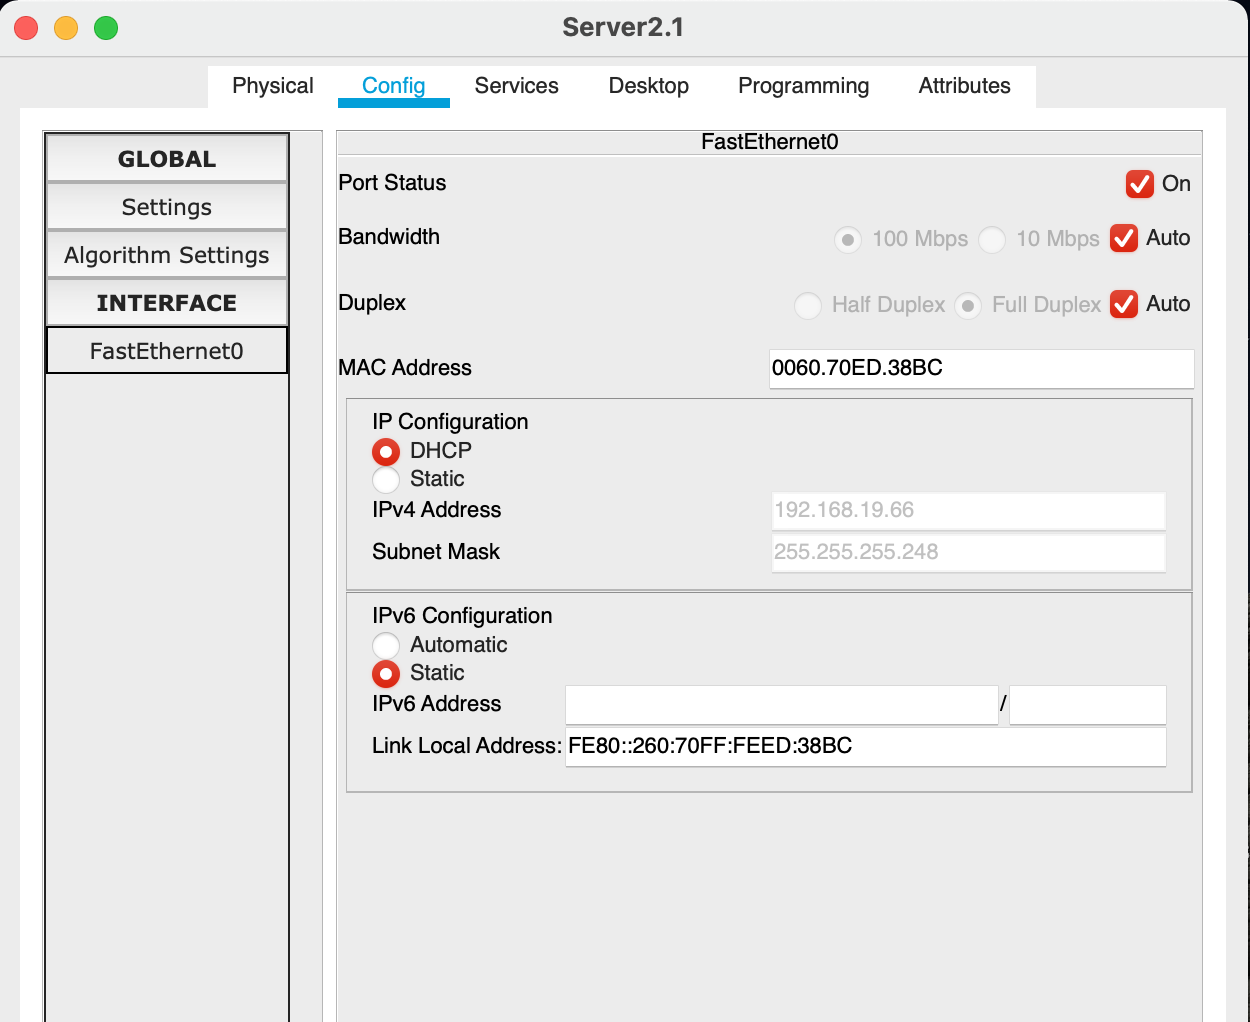
\includegraphics[width=0.5\textwidth]{img/content/PC_2.png}
    \caption{Автоматически выданный ip-адрес компьютера во второй подсети}
\end{figure}

\begin{figure}[H]
    \centering
    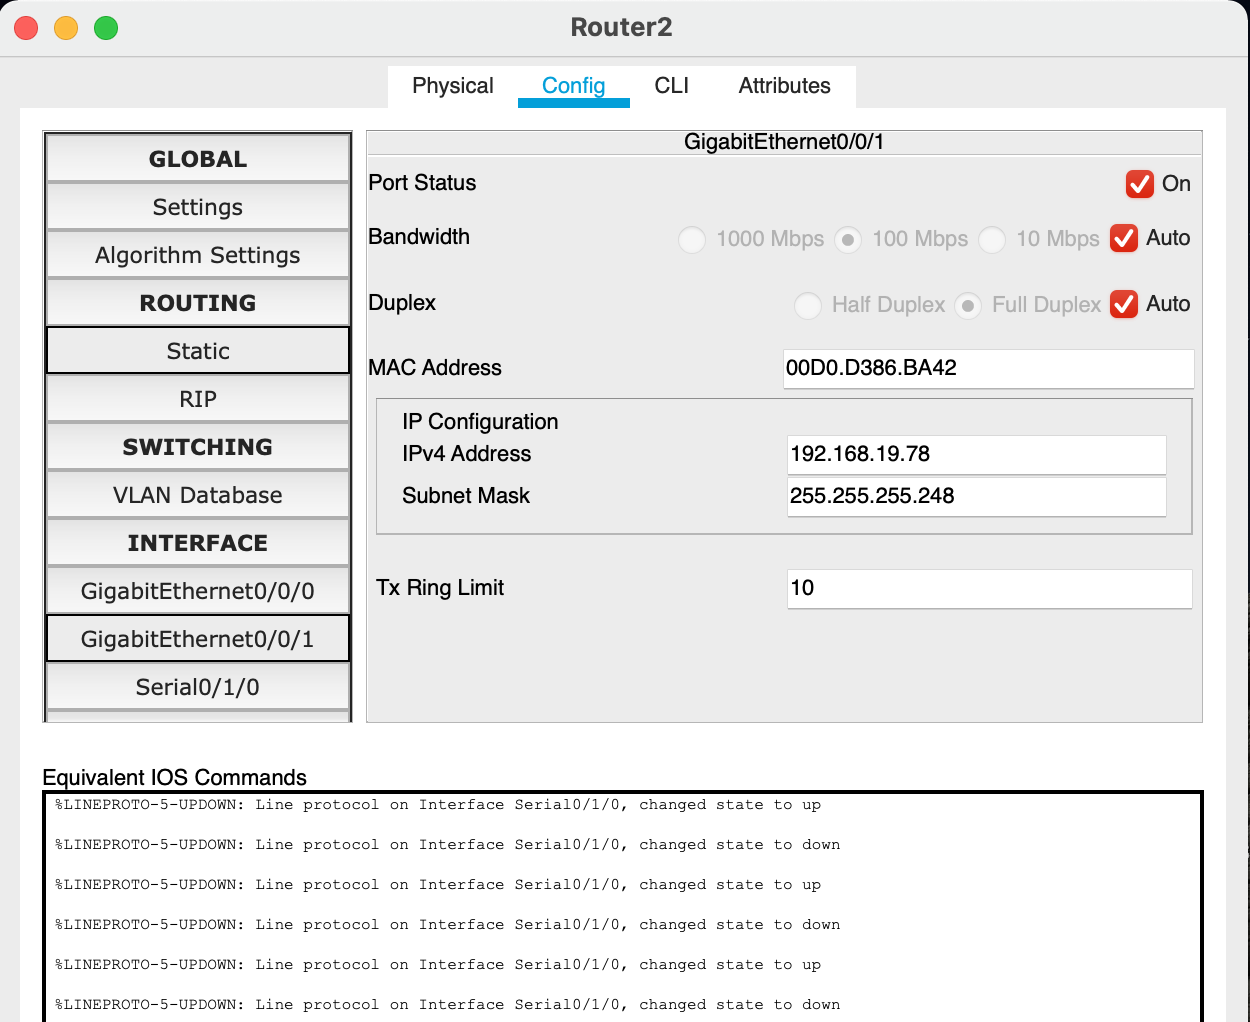
\includegraphics[width=0.5\textwidth]{img/content/DHCP_4.png}
    \caption{Настройка маршрутизатора в качестве DHCP-сервера для четвертой подсети}
\end{figure}

\begin{figure}[H]
    \centering
    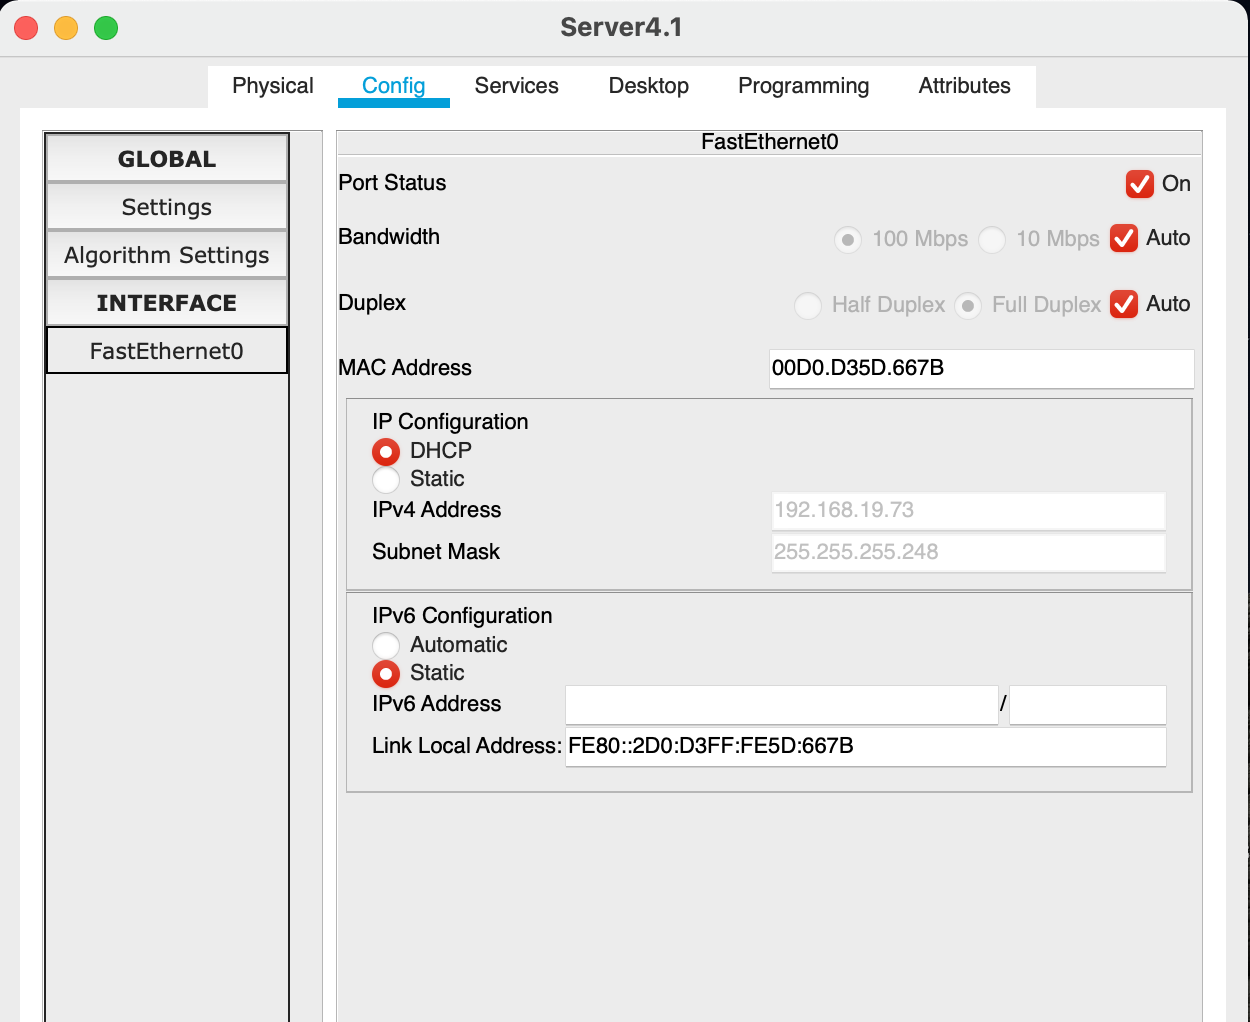
\includegraphics[width=0.5\textwidth]{img/content/PC_4.png}
    \caption{Автоматически выданный ip-адрес компьютера в четвертой подсети}
\end{figure}

\begin{figure}[H]
    \centering
    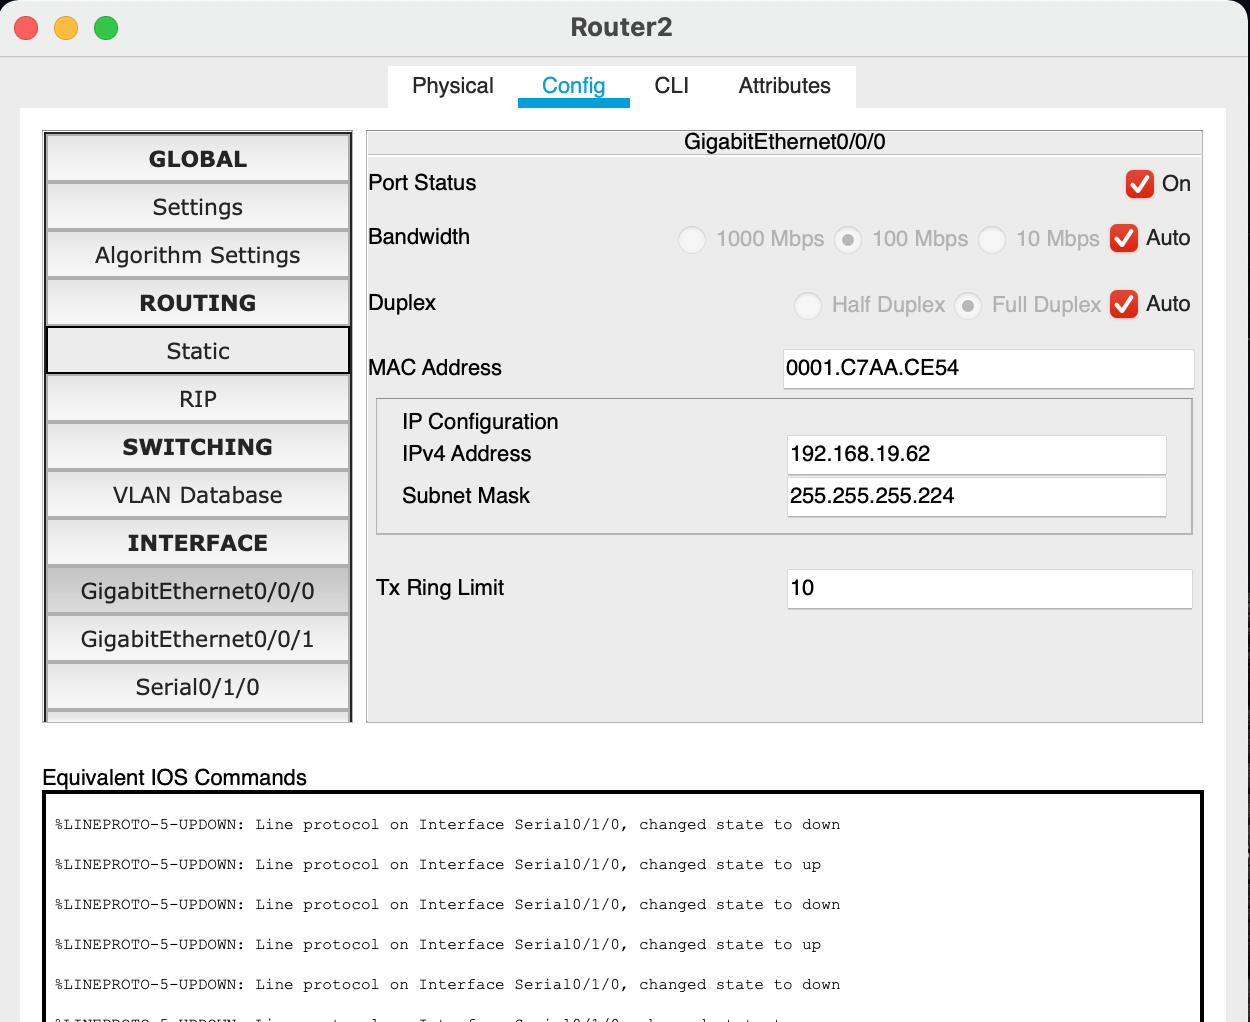
\includegraphics[width=0.5\textwidth]{img/content/DHCP_5.png}
    \caption{Настройка маршрутизатора в качестве DHCP-сервера для пятой подсети}
\end{figure}

\begin{figure}[H]
    \centering
    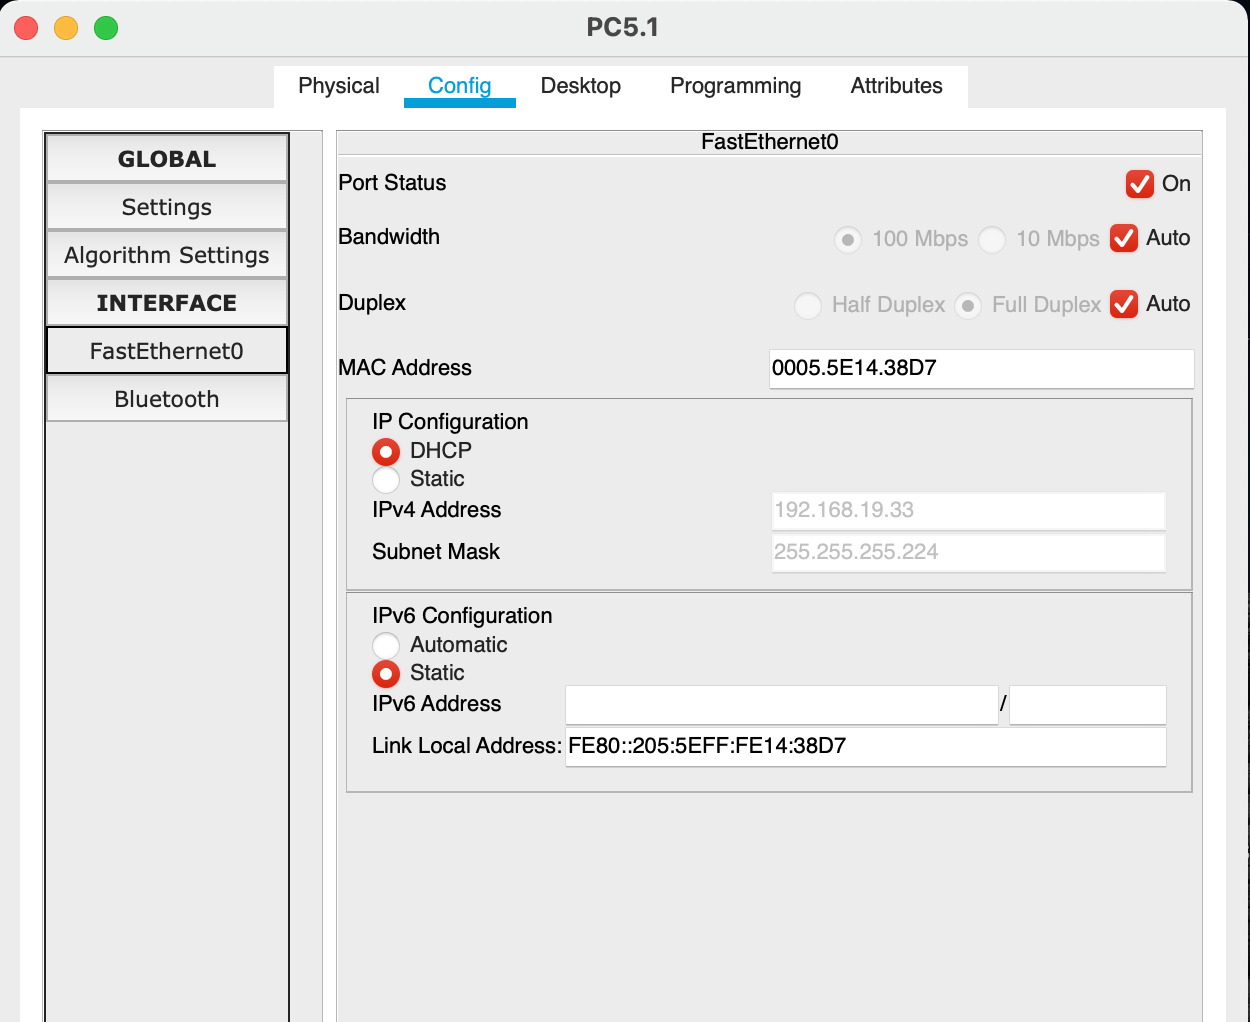
\includegraphics[width=0.5\textwidth]{img/content/PC_5.png}
    \caption{Автоматически выданный ip-адрес компьютера в пятой подсети}
\end{figure}

\begin{figure}[H]
    \centering
    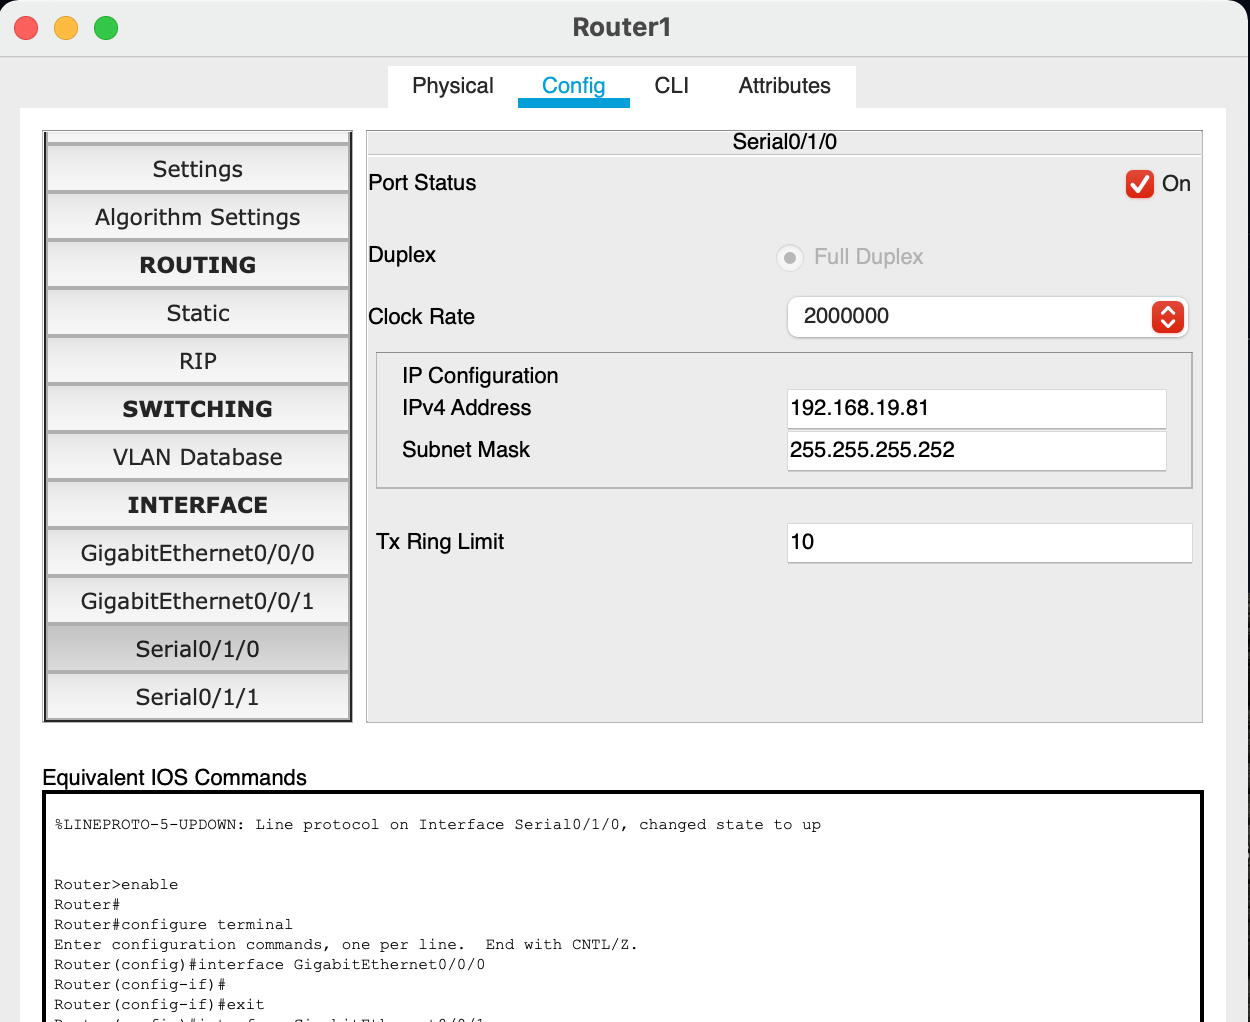
\includegraphics[width=0.5\textwidth]{img/content/DHCP_3_1.png}
    \caption{Настройка первого маршрутизатора для третьей подсети}
\end{figure}

\begin{figure}[H]
    \centering
    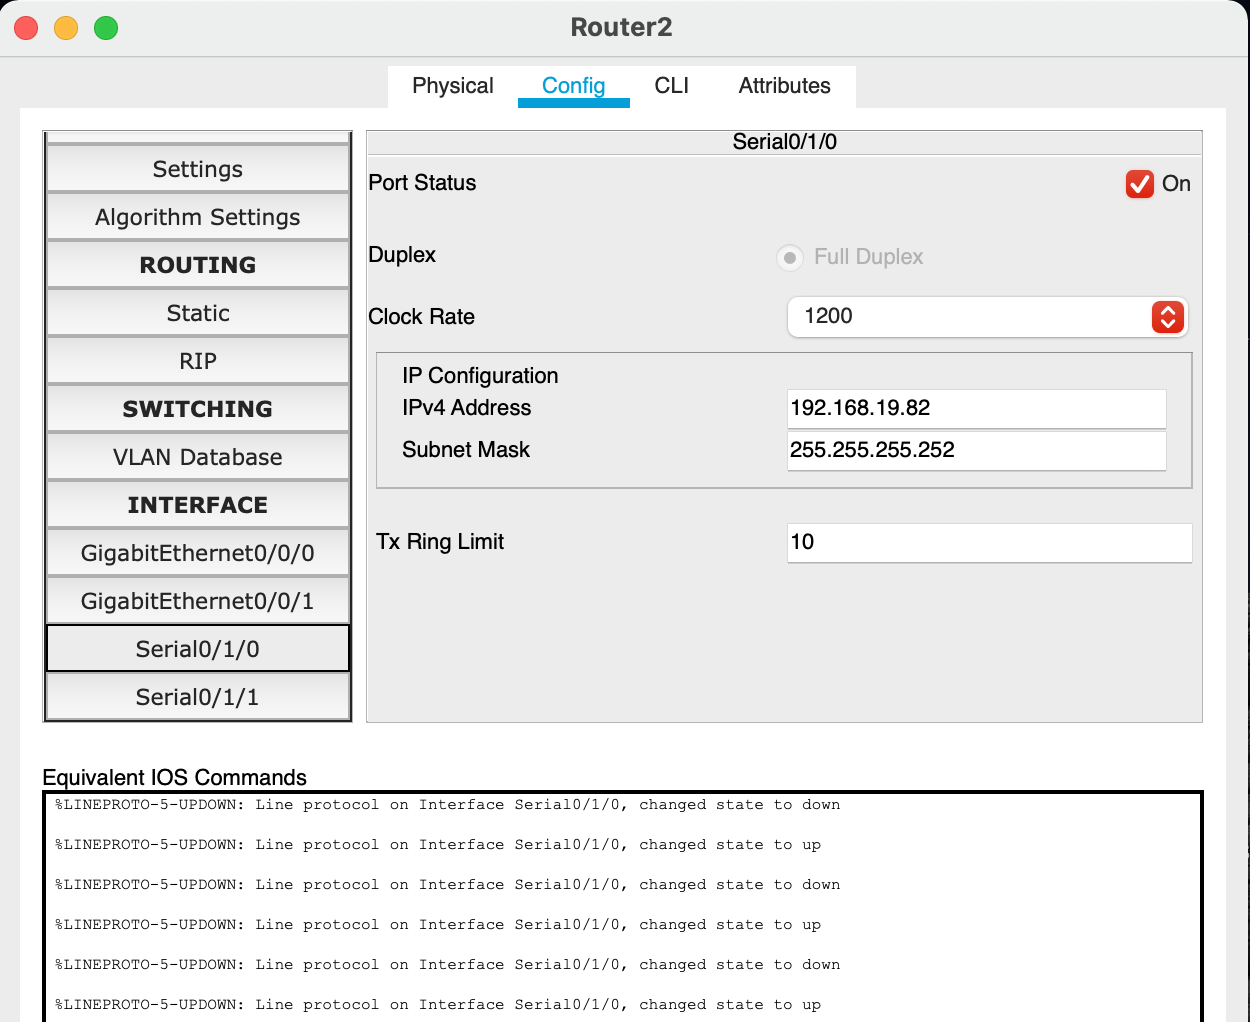
\includegraphics[width=0.5\textwidth]{img/content/DHCP_3_2.png}
    \caption{Настройка второго маршрутизатора для третьей подсети}
\end{figure}

\section{Проверка с помощью ping}

На рисунке \ref{fig:ping} показан рельтат работы двух команд ping с компьютера из первой подсети. Первая подсключается к адресу из той же подсети и выдает удачный результат. Во второй команде происходит попытка подключиться к адресу из другой подсети, попытка неудачна.

\begin{figure}[H]
    \centering
    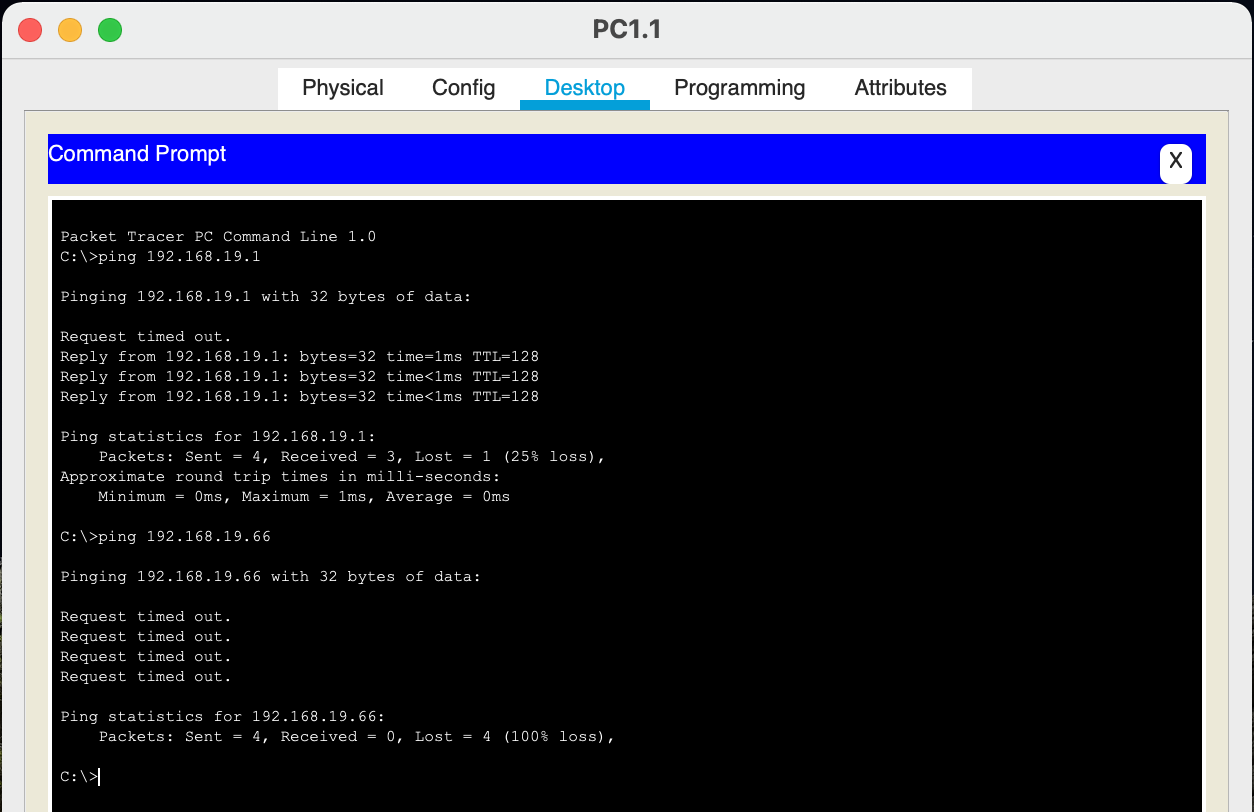
\includegraphics[width=0.5\textwidth]{img/content/ping.png}
    \caption{Попытка подключения к адресам}
    \label{fig:ping}
\end{figure}
